\section{Modeling Acceleration with Dependence-Graph Transformations} \label{sec:tdg}

This section describes our methodology for modeling acceleration, which
leverages the proposed transformable dependence graph (TDG).
We first give insight into the potential of dependence-based models, and discuss
background material.  We then describe how the TDG works, 
along with specific transformations and validation for five architectures, and conclude
by discussing the scope of the TDG.

\subsection{Why Dependence-Graphs?}
\paragraph{The Nature of Acceleration}
We first define an accelerator as: \emph{hardware which executes 
work in lieu of the general purpose processor to specialize elements 
of its execution}.  This means that the benefits and effectiveness of acceleration
depends what and how the general purpose processor gets specialized 
(\textbf{accelerator-specialization}),
the application for presenting certain characteristics which can be
specialized (\textbf{accelerator-application interaction}), 
and also in how the accelerator communicates with the 
core for coordination (\textbf{accelerator-core interaction}).  
Any effective model of acceleration must capture these three aspects.

%Therefore, a model for accelerators should have a 
%representation for both the elements of the general purpose processor
%which are being specialized, and also a model for the \emph{ways} in which they
%are being specialized by different accelerators.  

\paragraph{Dependence-Graph Models} 
Dependence-graph models are representations of the trace of execution for an architecture
running a specific application, which are composed micro-architectural events
as nodes, and dependences between events as edges~\cite{fields:isca01}.  Edges
have a weights that represent the latency between events, and represent phenomenon
like the issue width, ROB size, and data dependences.

The dependence graph is first of all a great candidate for accelerator modeling
because the dependence edges are exactly the aspects of general purpose cores
which can be specialized, and modeling this specialization is as simple as
eliding these edges (capturing accelerator-specialization).  Next, the
dependence graph itself is a representation of the program, containing all the
data and memory dependence information which characterizes it.  For this
reason, analyzing the program and the way the acceleration is affected by the
program is natural (capturing accelerator-application interaction).  Finally,
since the graph represents the execution at a sub-instruction granularity, the
communication between the accelerator and core can be modeled with simple
additional dependence edges (capturing accelerator-core interaction).

Therefore, 
the key to using dependence-graph models for acceleration lies in how to transform
the existing dependence graph representing general-purpose architectures to 
model the unique and varying phenomenon experienced by accelerators.

%\paragraph{Capturing Accelerator-Application Interactions}
%Applications and compilers have a profound influence on the ability
%of the accelerator to be effective, as accelerators rely on properties
%of the application through compiler analysis for correctness or suitability.
%For instance, if loop-level parallelism
%simply does not exist in an application, or the compiler cannot find it,
%then the effectiveness of SIMD acceleration is severely diminished. In this case,
%it would be important that the model captures this lack of acceleration opportunity.
%
%To appropriately model application and compiler interactions, the system must
%perform an analysis of the application's code and dynamic trace.  This
%analysis should ideally be optimistic, as the goal is to explore potential acceleration.
%We accomplish this by performing analysis directly on the trace of
%execution, rebuilding the original program's call graph, control flow graph, and
%data dependence graphs, and storing this as meta-information.  Further meta-information
%can be captured as per the requirements of each accelerator.
%
%\paragraph{Capturing Accelerator-Core Interactions}
%
%In order to capture fine-grained accelerator-core interactions, it is necessary to
%model the dependencies at the sub-instruction level.  This is because accelerators
%can be integrated at various levels.  SIMD accelerators are integrated directly
%into the pipeline, and thus their models should manipulate the processor's 
%events explicitly.  DySER is integrated into the pipeline, but 
%communicates through explicit instructions, and so its model should be 
%attached through operation complete events. 
%Conservation Cores, which communicates both through the pipeline and
%primarily through the memory system, must be modeled with dependencies at both levels.
%
%The dependence-graph naturally lends itself to fine grained interaction, with reasonably
%high abstraction.  Capturing accelerator-core interactions is a matter of applying
%the meta-information, stored along side the 
%dependence-graph as a result of previously mentioned trace
%analysis, and connecting, eliding, or reconnecting edges to model the dependencies
%inherent in accelerator architectures.  The nature of this analysis and these
%transformations are specific to each architecture, so we discuss the specifics in
%the following section.

\subsection{Overview}

\begin{figure}
  \begin{center}
    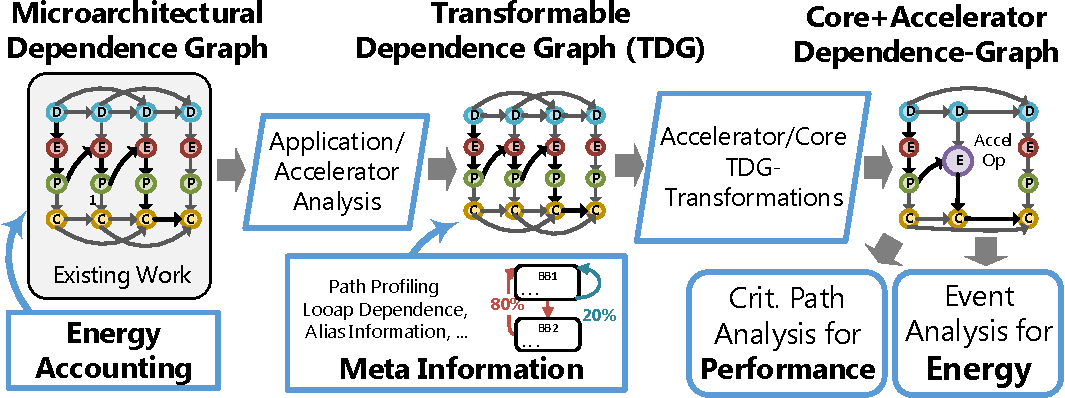
\includegraphics[width=0.77\linewidth]{figs/overview3.pdf}
  \end{center}
\vspace{-0.2in}
  \caption{Applying the Transformable Dependence Graph}
  \label{fig:overview}
\vspace{-0.05in}
\end{figure}

In this work, we propose a new abstraction, based on microarchitectural
dependence-graphs, for studying the nature of acceleration called the
\emph{transformable dependence-graph(TDG)}.  This abstraction augments the
original dependence-graph model with the ability to apply transformations
which model the dependencies inherent in various accelerators.
Figure~\ref{fig:overview} shows how our approach employs the TDG for modeling
acceleration.  First, we take an existing microarchitectural dependence-graph,
and augment it with annotations concerning the type of operation and accesses
it performs, which can be accumulated and used by existing power models to
calculate energy.  Next, an analysis pass determines specific application
properties, which we call \emph{meta-information}, to determine when it is
legal and beneficial to perform acceleration.  We then transform the graph
according to rules which model the accelerator's behavior, modifying or
inserting event nodes and dependency edges.  Using this transformed graph, we
determine the performance and the energy of the overall execution.

%Next, an analysis pass determines the properties about the application,
%accelerator-application interactions.  We then
%transform the graph according to rules which model the accelerator's behavior,
%modifying or inserting event nodes and dependency edges.  Using this transformed graph,
%we determine the performance and the energy of the overall execution.


\subsection{The Transformable Dependence Graph(TDG)}
\begin{figure}[tbp]
  \begin{center}
    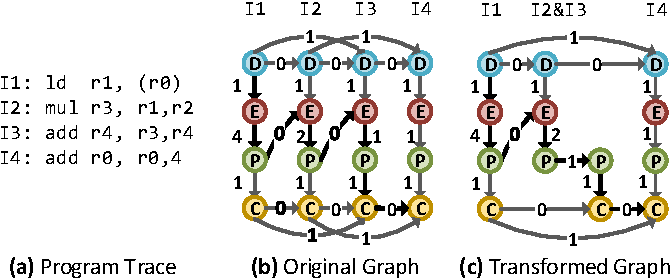
\includegraphics[width=0.6\linewidth]{figs/example.pdf}
  \end{center}
\vspace{-0.2in}
  \caption{Using the Transformable Dependence Graphs for modeling Custom Instructions. \newline
{\small
Edge descriptors in (a) and (b) indicate latency.
%, while in (c) they indicate energy events. 
Legend --  D: Dispatch, E: Execute, P: Complete, C: Commit
}}
  \label{fig:example}
\vspace{-0.05in}
\end{figure}

\paragraph{Microarchitectural Dependence-Graphs Background}
Microarchitectural dependence-graphs~\cite{fields:isca01}
represent the dynamic execution of processor pipelines abstractly.  
Nodes in the graph represent microarchitectural events,
and edges in the graph represent static and dynamic dependencies 
between events.  To give an example, 
Figure~\ref{fig:example}(a) shows a series of instructions, and 
Figure~\ref{fig:example}(b) shows a simplified dependence graph
representation of the execution for a two-wide out-of-order processor.

Nodes here represent different stages of the instruction's execution, 
like ``dispatch,'' ``execute,'' ``complete'' and ``commit.'' 
Edges represent dependences
which enforce constraints imposed by the architecture.  
To explain the diagram, edges 
between subsequent dispatch and commit nodes have a zero cycle latency,
and represent that both dispatch and commit must occur in order
($F_{i-1} \xrightarrow{_0} F_{i}$, $C_{i-1} \xrightarrow{_0} C_{i}$).  Edges between
alternate dispatch and commit nodes enforce the
issue width of the processor ($F_{i-2} \xrightarrow{_1} F_{i}$, $C_{i-2} \xrightarrow{_1} C_{i}$). 
The edge from execute to complete enforces
the latency of the operation or load ($E_{i} \rightarrow C_{i}$).  
Finally, data dependencies are edges between instructions, from 
 complete to execute ($P_{i} \xrightarrow{_0} E_{j}$).
By traversing edges through the graph, we compute the critical path and thus
the performance. 

\paragraph{Using the Dependence-Graph to Calculate Energy} One of our
contributions is to show how the microarchitectural dependence graph can be
used to calculate energy.  We take a quite straight forward approach in
associating appropriate energy events with each node.  For instance, the
dispatch node accesses the ROB, the execute node accesses specific functional
units (FUs), and so on.  As we traverse the dependence-graph, we calculate
the total event counts of each type.  Much like a simulator, we can feed these
event counts into established tools for energy/power estimates.

We also note that since the graph does not contain mis-speculated instructions, we
also must calculate the estimated number of additional events that would have occurred.
We do this by calculating the ratio of speculated to misspeculated instructions, and
multiplying the overall counts by this number.

\paragraph{Enabling Transformations to the Dependence-Graph}
The fundamental insight which we employ in this work is that accelerators,
which specialize elements of the processor's execution, can be modeled by
removing and transforming nodes and edges.  
Our evaluation shows that using the TDG, we
can achieve less than 15\% average error for all accelerators against published
or simulator data for both performance improvement and energy reduction.

To demonstrate this concept, we can consider adding a custom
multiply-accumulate instruction.  The TDG can capture this by recognizing this
computational pattern in the application, and eliding the dispatch and commit
nodes from the redundant instruction with a transformation.  Edges connecting
to the surrounding instructions are reattached to capture the pipeline
constraints, and Figure~\ref{fig:example}(c) shows the resulting graph.  What
enabled the transformation for the above example was the
\emph{meta-information} that the original two operations fit
%about the execution, particularly the fact that two dependent operations fit
the correct computational pattern. 
%This is a trivial example, in practice much more detailed application
%information is necessary.
In general, what makes the dependence graph ``transformable'' is having the
appropriate meta-information about both the semantics of operations and
properties of the dynamic execution.  Which meta-information is required
depends on the accelerator, and we discuss the next section.

\if 0
\subsection{Background on Accelerators}
Before we get into the details of the transformations of each accelerator, we need to
describe their basic principles.  A brief description of each is below.

\textbf{Conservation Cores}, is a structured hardware accelerator,
which automatically generates hardware implementations of application code.
By eschewing pipeline access with simple hardware, it is meant as an offload 
engine for energy efficiency.  
%Conservation Cores account for area required by
%choosing regions to maximize dynamic execution coverage while minimizing number of
%static instructions.

The \textbf{BERET} accelerator is also a structured-hardware accelerator,
essentially a trace processor for loops, where only the most frequently 
executed control path is executed in the accelerator.  
It targets energy efficiency by executing the hot path with compound functional 
units, called Serialized Execution Blocks (SEBs). 
Branch divergence entails re-execution on the main processor, 
after transferring buffered state.

\textbf{SIMD} acceleration relies heavily on exploiting independent loop iterations for
parallel execution, and is a well known acceleration strategy.  
%Though SIMD acceleration is a well known and
%has been studied extensively, understanding SIMD vectorization potential is still a challenge. 
%Our approach takes inspiration from Holewinski~\emph{et. al.} who also use dynamic
%traces~\cite{Holewinski:2012:DTA:2254064.2254108}.
%Our
%approach takes inspiration from Holewinski~\emph{et. al.} who also use dynamic
%traces~\cite{Holewinski:2012:DTA:2254064.2254108} to estimate vectorizable regions.  

\textbf{DySER} is a CGRA, operating in an access-execute fashion with the 
processor, accelerating the computational portions of the code.  
It is integrated with a vector interface to the host, enabling fast
streaming access and high energy efficiency.

\textbf{NPU} is a domain specific accelerator, meant to accelerate approximate
computations with neural networks(NNs).  It uses custom instructions for communication,
             and an access-execute model. 
It has a specialized buffer to cache re-used values, and a specialized
broadcast network.
\fi

 
\subsection{Accelerator TDG-Transformations} \label{sec:trans}

Here we describe how we modeled five specific accelerators through
applying TDG transformations.  These were chosen because they require
different program characteristics to be effective, which helps show how the TDG
can capture application-accelerator interactions.  Brief descriptions follow.

\textbf{Conservation Cores}, is a structured hardware accelerator,
which automatically generates hardware implementations of application code.
%By eschewing pipeline access with simple hardware, 
It is meant to be an offload engine for energy efficiency.  

The \textbf{BERET} accelerator is also a structured-hardware accelerator,
essentially a trace processor for loops, where only the most frequently 
executed control path is executed in the accelerator, using efficient compound
functional units called SEBs.
%It targets energy efficiency by executing the hot path with compound functional 
%units, called Serialized Execution Blocks (SEBs). 
%Branch divergence entails re-execution on the main processor, 
%after transferring buffered state.

\textbf{SIMD} acceleration relies heavily on exploiting independent loop iterations for
parallel execution, and is a well known acceleration strategy.  
%Though SIMD acceleration is a well known and
%has been studied extensively, understanding SIMD vectorization potential is still a challenge. 
%Our approach takes inspiration from Holewinski~\emph{et. al.} who also use dynamic
%traces~\cite{Holewinski:2012:DTA:2254064.2254108}.
%Our
%approach takes inspiration from Holewinski~\emph{et. al.} who also use dynamic
%traces~\cite{Holewinski:2012:DTA:2254064.2254108} to estimate vectorizable regions.  

\textbf{DySER} is a CGRA, operating in an access-execute fashion with the 
processor, accelerating the computational portions of the code.  
It is integrated with a vector interface to the host.
%, enabling fast streaming access and high energy efficiency.

\textbf{NPU} is a domain specific accelerator, meant to accelerate approximate
computations with neural networks(NNs).  It uses custom instructions for communication,
and an access-execute model. 
%It has a specialized buffer to cache re-used values, and a specialized
%broadcast network.

 

Table~\ref{tab:megametatrans}, describes the 
meta-information required and the TDG transformations for each accelerator.
Figure~\ref{fig:transformations} parallels this
description, showing an example for each accelerator.  
The original code has inner-control flow inside a loop, 
and also independent iterations.  On the right of the figure is the original
dependence-graph of four iterations of the dynamic execution. Each panel
shows accelerator-specific transformations.  

%In addition, we briefly describe
%the inorder transformations below.

\begin{table*}[h]
\begin{adjustwidth}{-0.6in}{-0.6in}
\begin{center}
\setlength{\tabcolsep}{.18em}
\def\arraystretch{0.0}
\footnotesize 
\begin{tabular}{m{0.02\linewidth}m{0.48\linewidth}m{0.48\linewidth}}

& \multicolumn{1}{c}{\textbf{Gathering Meta-Information}}
& \multicolumn{1}{c}{\textbf{TDG Transformations}}
\\   \midrule

\parbox[t]{1mm}{\rotatebox[origin=c]{90}{\textbf{Common}}} 
& 
\begin{itemize}
\item \textbf{CFG\&DFG}
Static CFG and dataflow graphs are built using the dynamic trace.  
The CFG is constructed by tracking BB boundaries, including branch targets.
\item \textbf{Loops}
Used dominator analysis to construct natural loops, and loop nests. 
\end{itemize}


& 
\begin{itemize}
\item \textbf{Processor Dependence Elision}
Most accelerator's offload instructions, so for these instructions,
their processor dependence nodes and edges are elided.

\item \textbf{Processor Instruction Elision}
Many $\mu$ops which the processor executes are not required in dataflow
based accelerators, like register moves, so they may be elided.

\end{itemize}
\\ [-0.6\normalbaselineskip]  \midrule

\parbox[t]{1mm}{\rotatebox[origin=c]{90}{\textbf{C-Cores}}} 
& 
\begin{itemize}
  \item \textbf{Loop/Func Frequency} Loop and function frequency is 
  derived from the dynamic trace of the program.
  \item \textbf{Selected Loops/Funcs} Region selection to cover
the maximum dynamic execution with fixed hardware budget.
Our heuristic walks the call tree, picking the most profitable loops and functions.
\end{itemize}
&
\begin{itemize}
\item \textbf{Basic Block Serialization}  As the accelerator is non-speculative,
basic blocks are serialized with additional edges between them. 
\item \textbf{Memory Serialization} Memory ops serialized in BBs.
\item \textbf{I/O Transfer} An edge is inserted between the Conservation
Core and the processor for transferring values, on entry/exit.
\end{itemize}

\\ [-0.6\normalbaselineskip]  \midrule

 
\parbox[t]{1mm}{\rotatebox[origin=c]{90}{\textbf{BERET}}} 
& 
\begin{itemize}
  \item \textbf{Path Profiles}
  BERET exploits loop path re-use, so we capture this application interaction with path-profiling~\cite{path-profiling}.  
  \item \textbf{SEB Partitions}
BERET maps hot-path code to limited \# of compound FUs(SEBs). 
Process modeled by fixed size subgraphs, optimized with integer linear programming.
\end{itemize}

&
\begin{itemize}
\item \textbf{Trace Construction}
BERET traces are constructed at appropriate loop heads, BBs serialized with
an additional node.
  \item \textbf{Region Configuration \& I/O Transfer}
Control transfer node models RF communication and configuration delay. 
\item \textbf{Instruction Replay}
On BERET misspeculation, the last iteration of the loop is replayed on the host.
\end{itemize}
\\  [-0.6\normalbaselineskip] \midrule


\parbox[t]{1mm}{\rotatebox[origin=c]{90}{\textbf{SIMD}}} 
&
  \begin{itemize}
  \item \textbf{Loop Dependence}
   We determine loop dependence by analyzing memory access through each loop-nest.
  \item \textbf{Alias Info}
  May/must alias information between memory operations.
  \item \textbf{Stride Analysis}
  To see if memory accesses follow a simple pattern which is vectorizable, we implement
  a per-operation memory access stride analysis, and determine the pattern.
  \end{itemize}
&
  \begin{itemize}
  \item \textbf{Loop Vectorization}
  Vector width number of iterations are coalesced.
  Peeled loops retain normal dependencies.
  \item \textbf{$\mu$op Splitting}
  Vector ops split for smaller vector lanes.
  \item \textbf{Control Flow Merging}
  Diverging control paths are merged in the TDG.  
  Static instructions are played reverse post order.
  \item \textbf{Mask Instruction Insertion}
  Mask instructions are inserted along merging control flow paths.
  \end{itemize}
 
\\  [-0.6\normalbaselineskip] \midrule

%\includegraphics[width=0.9\linewidth]{figs/limits-Energy-Delay-4.pdf} \\
%\includegraphics[width=0.9\linewidth]{figs/limits-Energy-Delay-5.pdf} \\

\parbox[t]{1mm}{\rotatebox[origin=c]{90}{\textbf{DySER}}} 
&
 \begin{itemize}
  \item \textbf{Program Dependence Graph (PDG)}
  The PDG is constructed by analyzing the CFG for control dependence.
  \item \textbf{PDG Slicing}
  The PDG is sliced according to heuristics, creating 
  a memory sub-region with loads, stores and dependent computation.
  The remaining computation is marked as the execute subregion.
  Subregions are only considered when communication costs are low.
\end{itemize}

& 
 \begin{itemize}
\item \textbf{Loop Vectorization}
Similar to the SIMD.
\item \textbf{Access-Execute Decoupling}
Communication instructions inserted at the borders of access 
and execute subgraphs.
\item \textbf{Configuration Insertion}
Configuration instructions (default 64), are inserted into the
main processor's pipeline when a new region is encountered.  Regions are
cached in 4-entry buffer until evicted.
\end{itemize}

\\ [-0.6\normalbaselineskip]  \midrule

\parbox[t]{1mm}{\rotatebox[origin=c]{90}{\textbf{NPU}}} 
&
\begin{itemize} 
  \item \textbf{Appproximable Regions} Marked by programmer.
  \item \textbf{Region inputs/outputs}
    Inputs and outputs of the candidate regions, both memory
    and registers, determined using existing meta-information.
\end{itemize}
&
\begin{itemize}
  \item \textbf{Region Elision and communication}
   Instructions from approximable region elided from main processor. 
   Execution is replaced with NPU invocation node, and communication
   edges added based on region inputs/outputs.
\end{itemize}
\\ [-0.6\normalbaselineskip]  \midrule



\parbox[t]{1mm}{\rotatebox[origin=c]{90}{\textbf{Inorder-Core}}} 
& 
\centering
\emph{none required}
& 
\begin{itemize}
\item \textbf{OOO Resource-Edge Removal} 
OOO resource dependences removed, branch penalty reduced.
\item \textbf{Serializing Execution} 
Inorder complete with: $P_{i-1} \xrightarrow{_0} P_{i}$.
%s enforced by adding edge
\item \textbf{Long Latency Operations}
Long latency operations stall the next execute node by the length of the pipeline.
\end{itemize}

\\ [-0.6\normalbaselineskip]  \bottomrule 

\end{tabular}

\caption{Description of Meta-Information and Graph Transformations}
\label{tab:megametatrans}  
\end{center}
\vspace{-0.15in}
\end{adjustwidth}

\end{table*}


\begin{figure*}
%  \begin{center}


\makebox[\textwidth][c]{
    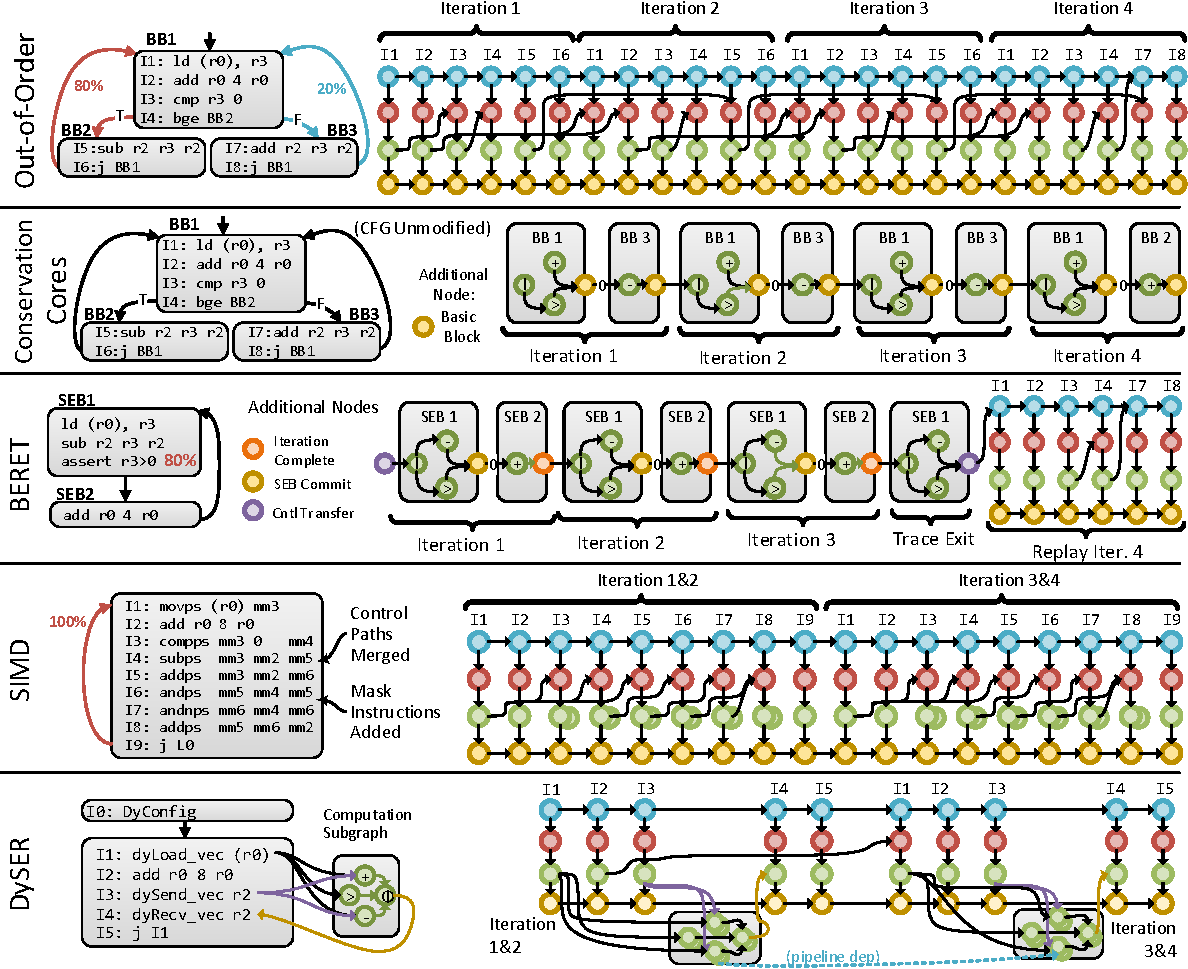
\includegraphics[width=1.19\linewidth]{figs/prism-transformations2.pdf}
}
%  \end{center}
  \vspace{-0.18in}
  \caption{Accelerator Dependence Graph Transformations}
  \label{fig:transformations}
\end{figure*}

\if 0

\paragraph{Common Analysis and Transformations}
The dataflow graph can be constructed by creating static representative instructions
and adding data dependencies between static instructions
as the trace is processed.  The CFG can be constructed by tracking
basic block boundaries, adding additional boundaries at the targets of branches.
Also, loop's are important for all accelerators, so
we construct natural loops using dominator analysis, and determine loop hierarchies.  
Figure~\ref{fig:transformations}(a) shows an example CFG loop with profiling 
information on the left.  On the right of the figure is the dependence-graph
of four iterations of the dynamic execution used to create this.  This particular loop
has inner-control flow, and also independent iterations, making it an interesting example
for our accelerators transformations in subsequent subsections.

Besides just the analysis, there are some common transformations which are applied
in most accelerators.
Since many accelerators offload entire instructions, the instruction-elision
 transformation is common.
Figure~\ref{fig:example}(c) shows an example of this, where instruction 3 is elided.
Subsequent instructions, like instruction 4, must detach the fixed pipeline edges
(like $F_{i-1} \xrightarrow{_0} F_{i}$, $C_{i-1} \xrightarrow{_0} C_{i}$,
$F_{i-2} \xrightarrow{_1} F_{i}$, $C_{i-2} \xrightarrow{_1} C_{i}$), and then re-attach
them according to the rules, according to how the pipeline execution has been altered. 

In the remainder of this section, we will discuss the accelerator specific 
meta-information and transformations, using Figure~\ref{fig:transformations} as our
example.

\paragraph{Conservation Cores}
%They are essentially hardware realizations of the programs CFG.  
%Since performance is similar
%to the baseline inorder core, Conservation Cores are best suited for improving
%the effeciency of heavily used memory-bound library code.

\subsubsection*{Meta-Information}
\begin{itemize}
  \item \textbf{Loop/Func Frequency} Analyzing the trace, we can determine the number of 
  static and dynamic instructions in loops and functions, which are the units of 
  granularity that Conservation Cores can accelerate.
  \item \textbf{Selected Loops/Funcs} This meta-information is determined by
``fitting'' the most dynamic instructions possible inside a certain area (based on
number of static instructions as an estimate).  This is similar to conventional
bin packing, except for the hierarchical nature of functions and loops.  Our
algorithm walks up the call tree along the most promising edges 
(highest dynamic to static instruction ratio).
\end{itemize}

\subsubsection*{Transformations}
\begin{itemize}
  \item \textbf{Processor Instruction Elision}  We first elide from the processor any instructions
  which are accelerated.  We keep only dataflow edges.
  \item \textbf{Basic Block Serialization}  As shown in Figure~\ref{fig:transformations},
  the accelerator is executed as a series of serialized basic blocks, because
  the execution is completely non-speculative.  A new node, having edges from
  the nodes at the end of the basic block to the start of nodes in the next basic block
  captures this.
  \item \textbf{Memory Serialization} Memory operations also serialized in BBs.
  \item \textbf{I/O Transfer} We create one final edge between the execution of the Conservation
  Core and the processor for transferring input arguments.
\end{itemize}

  
\paragraph{BERET}

The BERET accelerator, another example of the structured hardware accelerator class,
is essentially a trace processor for loops, where only the most frequently 
executed control flow path is executed in the accelerator.  
It targets energy efficiency by executing the hot path with compound functional 
units, called Serialized Execution Blocks (SEBs), which are configured once for
each loop. Combined with the fact
that BERET speculates only down the hot path, BERET eliminates the need
for the dynamic power dedicated to fetch and decode, branch predictors,
and many other power hungry structure accesses.
If the trace path is predicted incorrectly (\emph{i.e.} take a side branch),
the instructions must be replayed on the main processor, after transferring back the buffered state
from the previous iteration.


\subsubsection*{Meta-Information}
\begin{itemize}
  \item \textbf{Path Profiles}
  Since BERET requires path information for loops, we perform path profiling analysis on 
the execution trace according to Figure~\cite{path-profiling}.  
  \item \textbf{SEB Partitions}
  The loop's hot path must be mapped to the BERET compound functional units, or SEBs.  
  There are a fixed number of SEBs, of size ranging from 2 to 6 functions each, which
have specific connectivity based on workload characteristics.  To eliminate overspecialization
to the original benchmarks, we model their execution by using subgraphs of fixed size. 
We solve an integer linear program for each subregion to find the best subgraph-partitioning 
which minimizes the number of register reads and writes.
\end{itemize}

\subsubsection*{Transformations}
\begin{itemize}
  \item \textbf{Trace Construction}
  When a loop iteration begins, the entire generated loop-path for a single iteration is added,
which were determined during the analysis phase.  Individual SEBs are serialized
with an additional node, shown in yellow in the figure.  When the iteration is complete,
buffered stores are allowed to start begin.  As we process the dynamic trace, we
update the memory latency of the associated beret loads and stores.  When the
dynamic execution leaves the loop, we simply insert another control transfer node
connecting back to the main processor's fetch of the next instruction. 
  \item \textbf{Region Configuration \& I/O Transfer}
  When a loop which has a BERET 
accelerated version begins, we insert an edge to the control-transfer 
node(shown in purple in Figure~\ref{fig:transformations}), which represents 
the time to configure the accelerator. An additional
edge represents the data-transfer time for the initial values. 
  \item \textbf{Instruction Replay}
  If the dynamic trace doesn't take the hot path, we must replay the last iteration of the loop, and connect
an edge to the main processor's nodes from the SEB containing the compare which failed.
In the example in Figure~\ref{fig:transformations}, the branch is mispredicted, and 
we must replay iteration three on the main processor.
\end{itemize}


\paragraph{SIMD}
%SIMD acceleration is a well known and has been studied extensively, yet
%understanding SIMD acceleration potential is an important and difficult task.  Our
%approach takes inspiration from Holewinski~\emph{et. al.} who also use dynamic
%traces~\cite{Holewinski:2012:DTA:2254064.2254108} to estimate vectorizable regions.  
%SIMD acceleration relies heavily on exploiting independent loop iterations for
%creating vector instructions.  Our analysis and transformations are described below.

\subsubsection*{Meta-Information}
\begin{itemize}
  \item \textbf{Loop Dependence}
   We determine loop dependence by analyzing memory access through each loop-nest.
  \item \textbf{Alias Info}
  To help determine loop dependence, we 
  also determine may/must alias information between memory operations.
  \item \textbf{Stride Analysis}
  To see if memory accesses follow a simple pattern which is vectorizable, we implement
  a per-operation memory access stride analysis, and determine the pattern.
\end{itemize}

\subsubsection*{Transformations}
\begin{itemize}
  \item \textbf{Loop Vectorization}
  SIMD performs loop vectorization where it is legal, as per the meta-information. 
  In practice we play the static instructions into the model, but update them with 
  the dynamic events like branch mispredictions and the induced memory latency.
  \item \textbf{SIMD $\mu$op Splitting}
  Because the implementation of SIMD which we validate against splits vector operations
  into multiple smaller $\mu$ops, we also perform this transformation based on
  the opcode by inserting additional instructions.
  \item \textbf{Control Flow Merging}
  When loops have multiple paths, SIMD must execute both paths and merge the
  results together.  We play static instructions through loops in RPO (reverse post order).
  \item \textbf{Mask Instruction Insertion}
  Mask instructions inserted along merging control flow paths for values updated
  in both paths, which is similar to phi insertion.
\end{itemize}



\paragraph{DySER}
DySER is a dataflow engine operating in an access-execute fashion with the 
main processor, accelerating the computational portions of the code.  
It is integrated in much the same way a SIMD unit would be, enabling vectorized access
through loads, stores, and register moves.  It's substrate, which
consists of functional units (FUs) and switches, forms a statically 
routed network, which is configured for each region of interest. A profiler 
or programmer determines the most commonly executed regions, and the 
code is sliced into the access subgraph (executes on the CPU) and the 
execute subgraph (executes on DySER).  Communication instructions are 
used for communication.

\subsubsection*{Meta-Information}
\begin{itemize}
  \item \textbf{Program Dependence Graph (PDG)}
  The PDG is constructed by analyzing the CFG for control dependence,
  using established techniques.
  \item \textbf{PDG Slicing}
  The PDG is sliced according to published heuristics used by the DySER
  implementers, creating a memory sub-region with loads, stores and dependent
  computation.  The remaining computation is marked as the execute subgregion.
  Subregions are only marked where thought to be beneficial, as excess communication
  can cause slowdown.
\end{itemize}

\subsubsection*{Transformations}
\begin{itemize}
\item \textbf{Loop Vectorization}
Loop vectorization works similarly to the SIMD case, except that the addition
of the configurable network allows some dependent loops to be vectorized as well.
\item \textbf{Access-Execute Decoupling}
Communication instructions are inserted at the borders of the determined access 
and execute subgraphs.
\item \textbf{Configuration Insertion}
Additional configuration instructions (default 64), are inserted into the
main processor's pipeline when a configuration is required.  Subsequent iterations
of the same accelerated region do not need to be reconfigured, as they are cached.
\end{itemize}

\paragraph{NPU: Neural Processing Unit}
NPU~\cite{npu} is a reconfigurable accelerator, tightly
coupled to the processor pipeline to accelerate multi-layer neural
network(NN). NPU contains 8 identical processing engine (PE) which
computes $sigmoid(\Sigma_i(x_i \times w_i))$, where $x_i$ is the input
to a neuron, $w_i$ is the corresponding weight. It has weight buffer
to cache the weights and a specialized broadcast network.
NPU acceleration starts with programmer
identified code regions or functions that can be approximated with NN.
After the NN is trained, the NPU compiler generates configuration for
NPU configuration, which
specifies the weights and the order of operations for the PEs, to implement
the trained multi-layered NN.  Similar
to DySER, NPU communicates to the processor through FIFOs.

\subsubsection*{Meta Information}
\begin{itemize}
  \item \textbf{Appproximable Regions}
    NPU acceleration heavily rely on the programmer's ability to
    identify the functions that can be approximated. Similarly, we
    determine the function boundaries with call/ret instructions.
  \item \textbf{Region inputs/outputs}
    We determine the inputs and outputs of the candidate regions, both memory
    and registers.
\end{itemize}

\subsubsection*{Transformations}
\begin{itemize}
  \item \textbf{Region Elision and communication}
   Similar to conservation cores transformation, we first elide all
   instructions in the region from the processor and it is replaced
   with NPU communication instruction and NPU invocation. In addition,
   it uses the similar transformation of CCores to manage the inputs and outputs
   from NPU.
\end{itemize}

\fi


%\paragraph{Inorder Dependence-graph Transformations}
%We also model inorder cores through TDG transformations:
%
%%\subsubsection*{Transformations}
%\begin{itemize}
%\item \textbf{OOO Resource-Edge Removal} 
%Dependence-edges modeling OOO structures are removed, and the 
%branch misprediction penalty is reduced.
%\item \textbf{Serializing Execution} 
%Inorder complete is enforced by adding edges: $P_{i-1} \xrightarrow{_0} P_{i}$.
%\item \textbf{Long Latency Operations}
%Long latency operations stall the next execute node by the length of the pipeline.
%\end{itemize}

%\input{tables/other-accel-meta-trans} 

%\paragraph{Others} 
%Our transformable dependence graph model can also be 
%used to model accelerators other than what we evaluate.
%Table~\ref{tab:other-metatrans}(Page~\pageref{tab:other-metatrans}) shows the
%summary of meta information and transformations needed to study diverse
%accelerators proposed.

\subsection{Implementation - Prism}
Our implementation of the transformable dependence-graph (TDG) is 
called \emph{Prism}.  We first describe the implementation
of Prism, how it integrates with the simulator and energy analysis
tool, and then describe the details of the nodes and 
edges we use to model microarchitectural dependence. %Then, we present the validation of the out-of-order model
%with a set of customized stress-test benchmarks, and validate each
%accelerator against simulated or published data.  

\if 0
\begin{figure}
  \begin{center}
    \includegraphics[width=\linewidth]{figs/marketing_diagram.pdf}
  \end{center}
  \caption{High-level Prism Implementation}
  \label{fig:prism}
\end{figure}
\fi

\paragraph{Simulator Instrumentation}
Prism generates the original dependence graph using gem5~\cite{gem5}.
We gather five pieces of information from the simulator: 
1. A description of the static instruction for each dynamic;
2. The dynamic dependencies between instructions (register \& memory);
3. The dynamic memory latencies;
4. Branch mispredicts; and
5. Memory addresses.
Any other source of this set of information would be sufficient
for building the TDG.

\paragraph{Generating Meta-Information and Prism Transformations}
The second phase of our approach is to generate meta-information
by analyzing the trace, acting like an optimistic compiler analysis.
A final pass is performed over the TDG, and 
it is then transformed to model different accelerators, 
as described by Section~\ref{sec:trans}.  
The cycle counts are computed dynamically by traversing the
critical path of the graph.

\paragraph{Energy Models}
Prism energy models work by first accumulating appropriate energy event counts for both
the main processor and also for the accelerator as the TDG is being transformed into core
and accelerator components.  At the end of the
transformation, we have two sets of activity counts.  The core activity counts
are fed to McPAT~\cite{mcpat} for processor power/energy.  
For the accelerator events, to make
the comparison between accelerators as fair as possible, we let McPAT handle
common energy components (FUs, reg-files, etc), which it is designed
for.  We also account for accelerator specific hardware, using per-access
energy estimates based on existing publications.


\paragraph{Prism's Dependence Graphs}
%We have thus far abstracted away most of the details of the baseline out-of-order
%model, primarily because the transformations described in earlier sections are mostly
%independent of the particular edges used to model the main processor. 
 Table~\ref{tab:inst-nodes} shows the nodes that we use to model processor instructions
in Prism, and also the intra-instruction edges and their latencies.  
Highlighted rows are additions to the model of Fields et al.~\cite{fields:micro03}. 
 The biggest difference is the addition of
Fetch and Writeback nodes to model front-end pipeline stalls and memory bandwidth
respectively.

Of primary note is the additions of the
fetch nodes and, for stores, writeback nodes.  Fetch nodes were added primarily
because it eases the addition of various pipeline stalls.  For instance, LSQ full events
stall in the dispatch stage, but control misspredictions stall at the fetch stage.
Writeback nodes are useful for modeling serialization instructions, and for modeling
store bandwidth.  In terms of edges between nodes inside instructions, there are other 
differences to the previous models in the literature.  For instance,
Prism uses architectural parameters for operation latency and throughput rather than recorded
values from the trace, and also we eliminate the latency of cache-line dependent loads, because this
recorded latency is simply an artifact of the when the cache-line dependent load happened
to get fired.  These modifications improve the graphs ability to be accurate when other events
are sped up.

Table~\ref{tab:prism-edges} details the static and dynamic edges that are placed
between instructions in prism.  Here, static means that the edge is static with
respect to the trace of execution.  Dynamic edges refer to those for which it 
is not known where the dependence should be placed before execution reaches
that point, occurring because of resource constraints.  For these cases, we add
to the graph model some additional logic to compute resource usage.
The implication is that static edges can be placed independently of any other
edge.  Most edges in this category are similar to previous works, but Prism
includes a few additional edge types.  Because we added a fetch node, Prism
includes an additional edge to model frontend pipeline buffering.  Also, we
implemented edges to constrain the load and store queues, and for the
non-speculative and serializing instructions.

%Modified from
\definecolor{CNew}{rgb}{1,.9,.9}
\definecolor{CMod}{rgb}{1,.9,.9}

\begin{table}[tbp]
  \begin{center}
  \begin{minipage}{0.25\linewidth}

  \begin{center}
    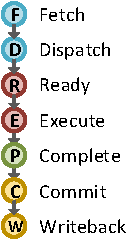
\includegraphics[width=0.4\linewidth]{figs/inst-nodes.pdf}
  \end{center}

  \end{minipage}\quad
  \begin{minipage}{0.6\linewidth}
    \scriptsize
    \setlength{\tabcolsep}{.19em}
    \def\arraystretch{1.1} 

    \begin{tabular}{llll}\toprule
       \textbf{Edge} & \textbf{Constraint} & \textbf{Latency}\\ \midrule
\rowcolor{CNew}
         $F \rightarrow D$         & Frontend Pipeline Latency & Fixed Lat. \\
         $D \rightarrow R$         & Dispatch Before Ready & 0 \\
         $R \rightarrow E$         & Ready Before Execute & 0 \\ 
         $E \rightarrow P$         & Execution Latency & Fixed, based on Op. \\
         $E \rightarrow P$         & Load Latency & Recorded Load Lat. \\
         $P \rightarrow C$         & Complete before Commit & Fixed Lat. \\
\rowcolor{CNew}
         $C \rightarrow W$         & Commit Before Writeback & Recorded Store Lat. \\ 
      \bottomrule
    \end{tabular}


  \end{minipage}
\end{center}
\vspace{-0.2in}
\caption{Prism Instruction Nodes and Edges}
\label{tab:inst-nodes}
\vspace{-0.1in}
\end{table}

\begin{table}
\begin{center}

\scriptsize
\def\arraystretch{0.9}
\setlength{\tabcolsep}{.19em}
    \begin{tabular}{llll}  \toprule
    \textbf{Static Edge} & \textbf{Constraint} & \textbf{Latency} \\ \midrule
    $F_{i-1}\rightarrow F_{i}$ & Fetch In-order & 0 \\
    $D_{i-1}\rightarrow D_{i}$ & Dispatch In-order & 0 \\
    $C_{i-1}\rightarrow C_{i}$ & Commit In-order & 0 \\ 
    $F_{i-fw}\rightarrow F_{i}$ & $fw=~$Fetch Width & 1 \\
    $D_{i-dw}\rightarrow D_{i}$ & $dw=~$Dispatch Width & 1 \\
    $C_{i-cw}\rightarrow C_{i}$ & $cw=~$Commit Width & 1 \\ 
    $F_{i-1}\rightarrow F_{i}$ & Icache Latency & Recorded \\


\rowcolor{CNew}
    $D_{i-ibuf\_sz}\rightarrow F_{i}$ & $ibuf\_sz=~$ Frontend Pipeline Buffer Size & 0 \\

    $C_{i-{rob\_sz}}\rightarrow D_{i}$ & $rob\_sz=~$ Reorder Buffer Size  & 0 \\ 

    $P_{i}\rightarrow R_{j}$ & Data Dependence, apply if Inst$_j$ depends on Inst$_i$ & 0 \\ 
    $P_{i}\rightarrow R_{j}$ & Mem Dependence, apply if Inst$_j$ mem depends on Inst$_i$ & 0 \\ 

\rowcolor{CNew}
    $P_{i}\rightarrow D_{j}$ & LQ Size, apply if Inst$_j$ is $lq\_size$ loads after Inst$_i$ & 0 \\ 
\rowcolor{CNew}
    $P_{i}\rightarrow D_{j}$ & SQ Size, apply if Inst$_j$ is $sq\_size$ stores after Inst$_i$ & 0 \\ 

\rowcolor{CNew}
    $C_{i}\rightarrow F_{i+1}$ & Inst$_i$ is serializing & 0 \\ 
\rowcolor{CNew}
    $W_{i}\rightarrow R_{j}$ & Inst$_j$ is non-speculative, and Inst$_{i}$ is the previous store  & 0 \\ 

    $C_{i}\rightarrow F_{i+1}$ & Ctrl Inst$_i$ mispredicted, Inst$_{i+1}$ waits until rob is flushed. & Estimated \\

    $P_{i}\rightarrow P_{j}$ & Load Inst$_i$ pulls cache line for Load Inst$_j$. & 0 \\
    
\bottomrule
\toprule
  \textbf{Dynamic Edge} & \textbf{Constraint \& Latency} \\ \midrule
\rowcolor{CNew}
    $E_{i}\rightarrow D_{j}$ & IW Size, apply if Inst$_i$ blocks Inst$_j$ from the IW & 1 \\
    $E_{i}\rightarrow E_{j}$ & Execution Resource Conflict & 1 \\
\rowcolor{CNew}
    $P_{i}\rightarrow F_{j}$ & Load Inst$_j$ blocks in the cache b/c of Inst$_i$, requires pipe flush.  & 1 \\ 
\rowcolor{CNew}
    $W_{i}\rightarrow W_{j}$ & L1 Cache B/W, apply if $W_j$ can enter L1 after $W_i$  & 1 \\

\bottomrule
\end{tabular}

\caption{Static and Dynamic Inter-Instruction Edges}
\label{tab:prism-edges}
\end{center}

\vspace{-0.05in}
\end{table}


%, including the instruction window, execution units, and MSHRs in the l1 cache.
%The alternative to dynamically adding these edges is to make a static prediction
%based on the given execution, but we found this was not flexible when transforming
%the event graph, leading to under-predictions.



\begin{figure}
\begin{adjustwidth}{-0.75in}{-0.75in}
\begin{center}
\footnotesize
\def\arraystretch{0.25}
\begin{tabular}{cccc}
%   \multicolumn{2}{ c }{stuff}  \\ \toprule
%   \multicolumn{1}{ c }{\textbf{Performance}} & \multicolumn{1}{ r }{\textbf{Energy}}  \\ \toprule
%Performance & Energy \\ \toprule

\textbf{~~~~~~~~~~~~~~~~~~Performance} & \textbf{~~~~~~~~~~~~~~Energy} &
\textbf{~~~~~~~~~~~~~~~~~~Performance} & \textbf{~~~~~~~~~~~~~~Energy} \\ \toprule
    \multicolumn{2}{ c }{(a) 1-Wide OOO Processor (from 8 wide simulation)} &
    \multicolumn{2}{ c }{(b) 8-Wide OOO Processor (from 1 wide simulation)} \\

    \multicolumn{2}{ c }{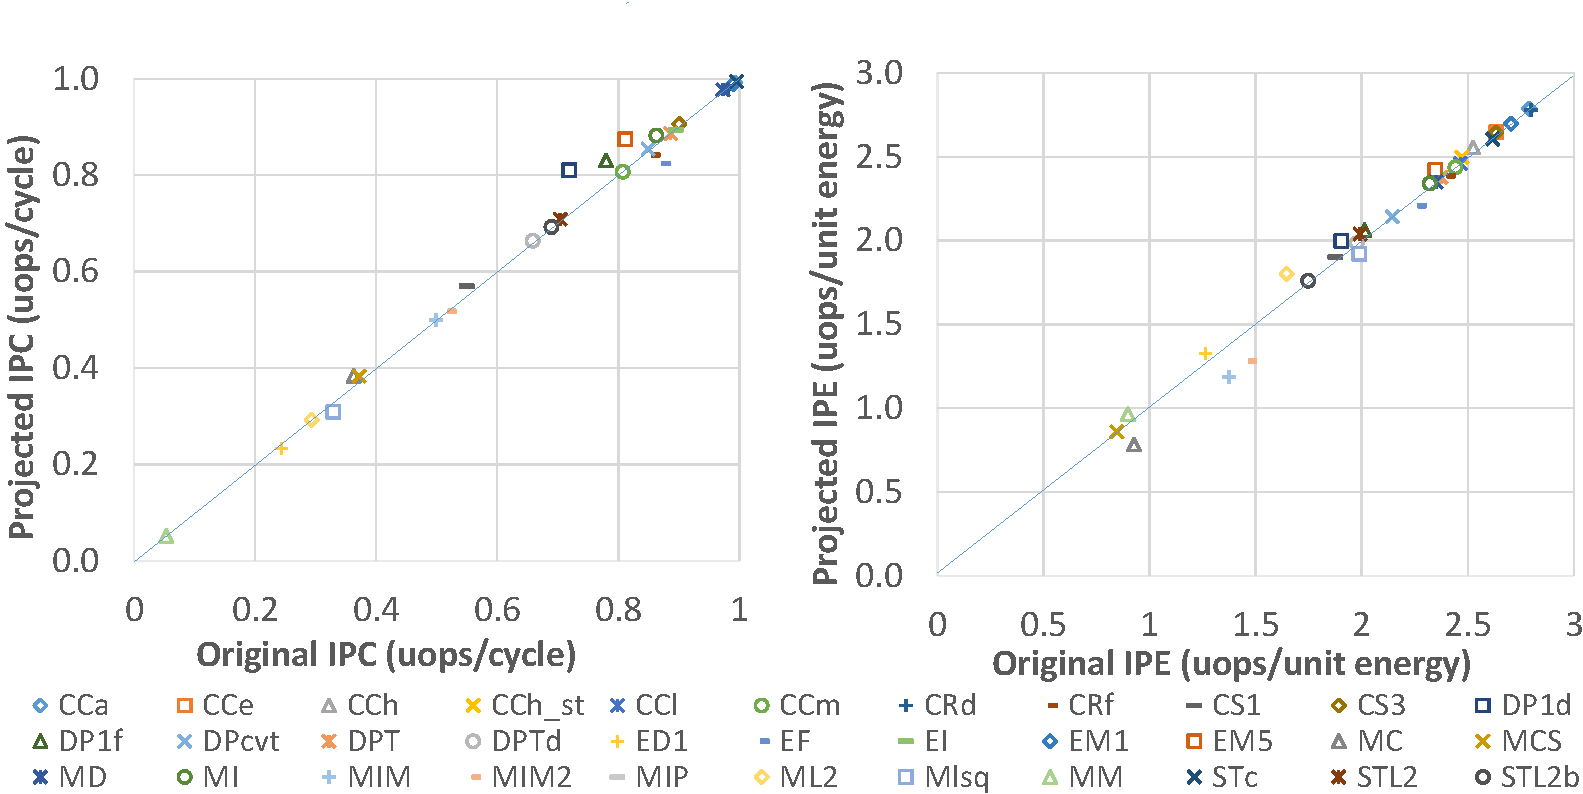
\includegraphics[width=0.44\linewidth]{figs/v_ooo_8to1.pdf}} &
    \multicolumn{2}{ c }{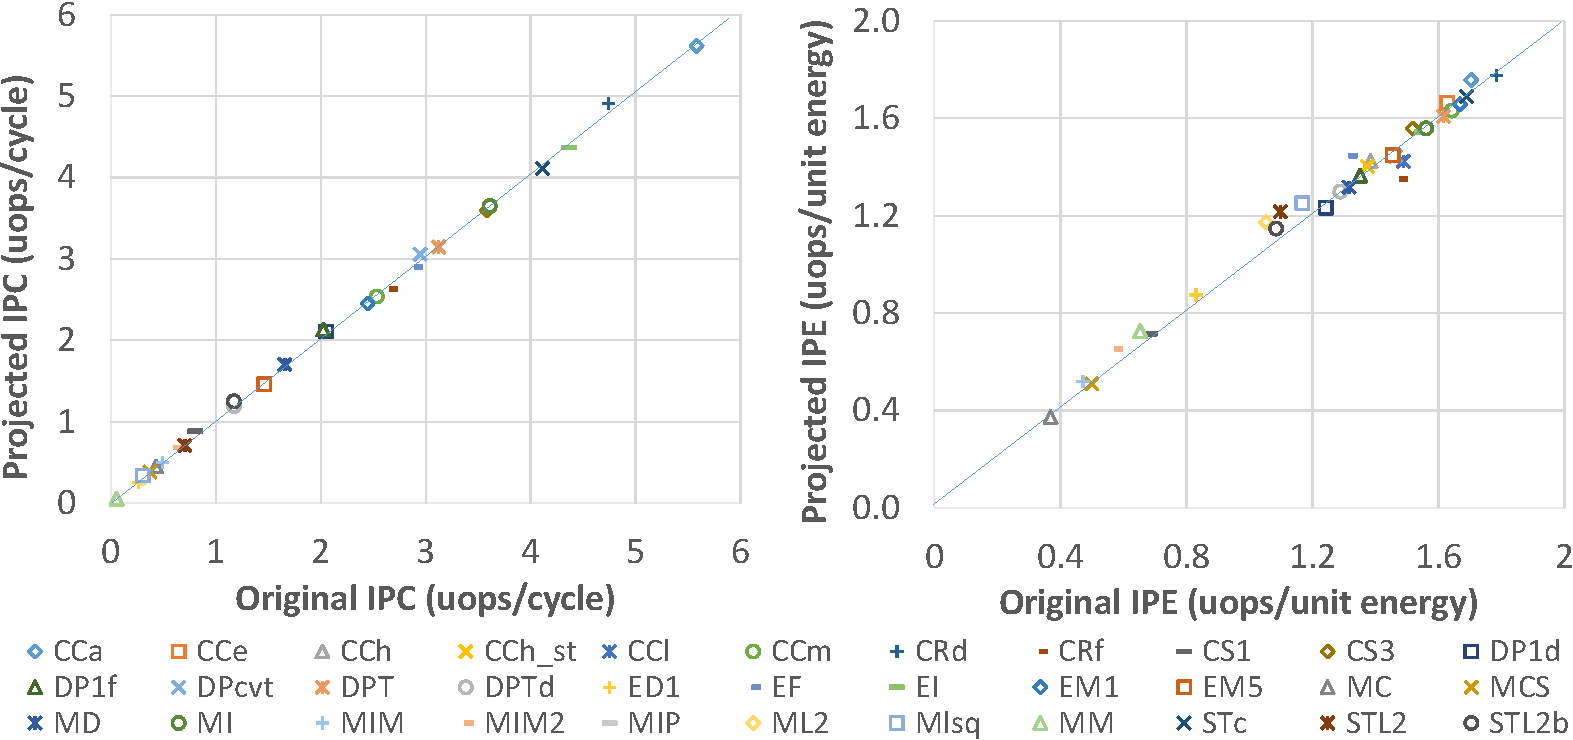
\includegraphics[width=0.44\linewidth]{figs/v_ooo_1to8.pdf}} \\
    \midrule

    \multicolumn{2}{ c }{(c) Conservation Cores} &
    \multicolumn{2}{ c }{(d) BERET} \\

    \multicolumn{2}{ c }{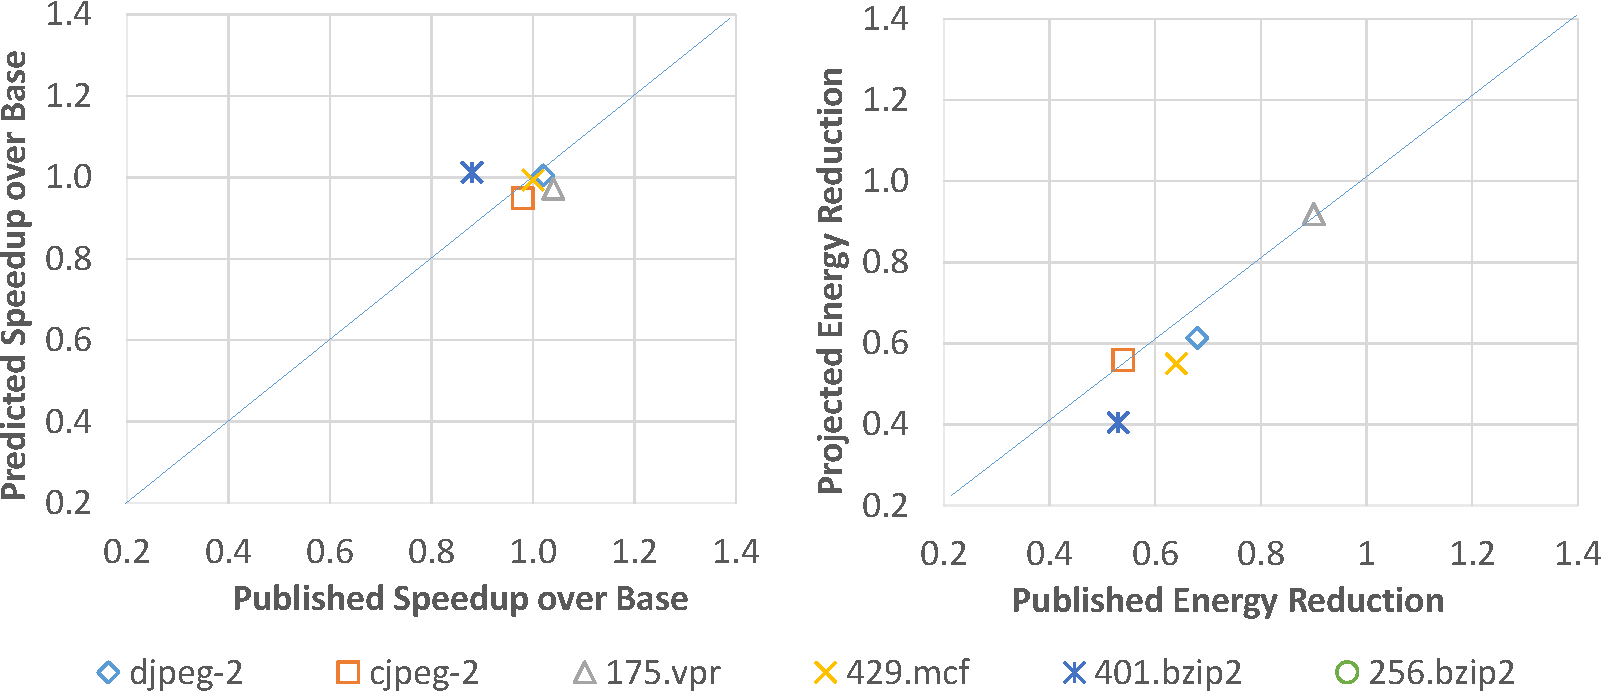
\includegraphics[width=0.44\linewidth]{figs/v_ccores.pdf}} &
    \multicolumn{2}{ c }{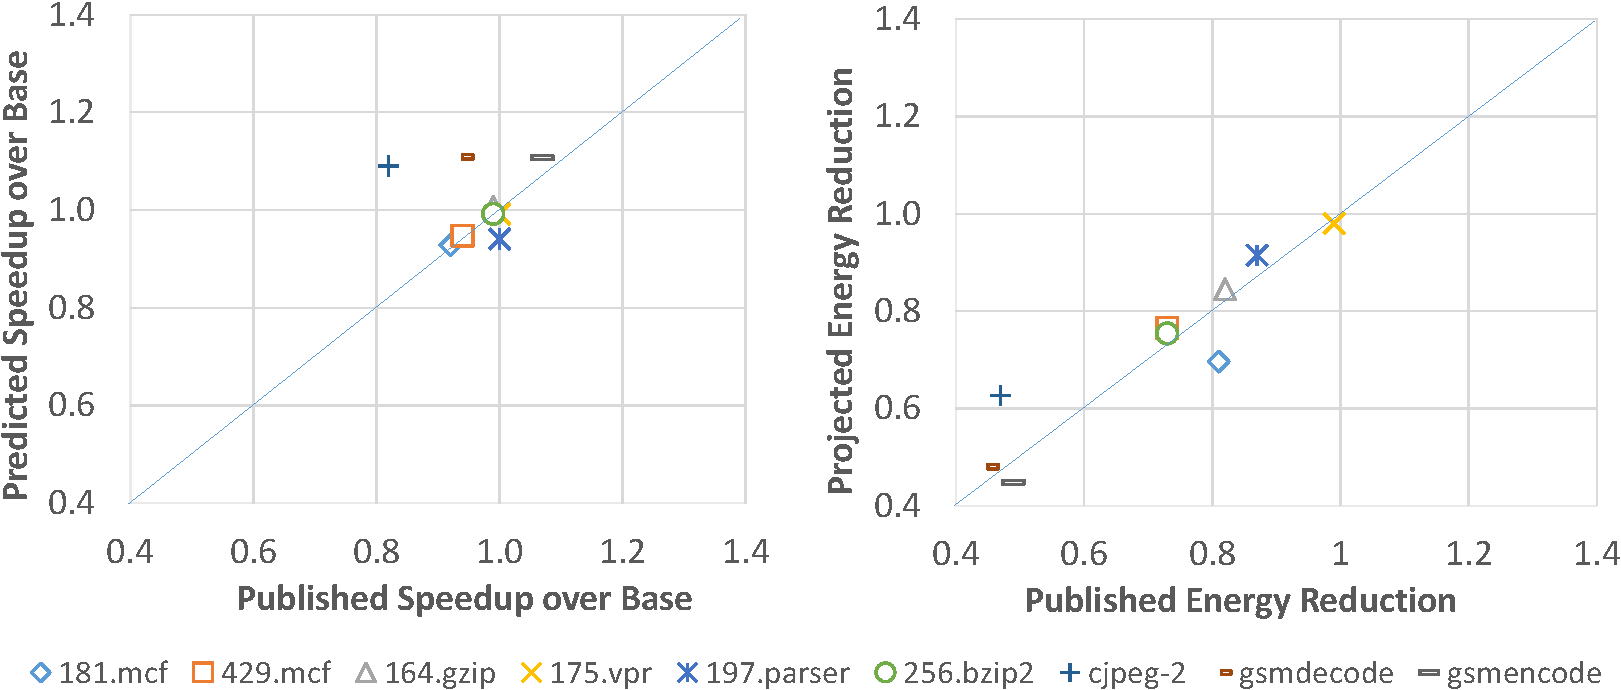
\includegraphics[width=0.44\linewidth]{figs/v_beret.pdf}} \\
    \midrule

    \multicolumn{2}{ c }{(e) SIMD} &
    \multicolumn{2}{ c }{(e) DySER} \\

    \multicolumn{2}{ c }{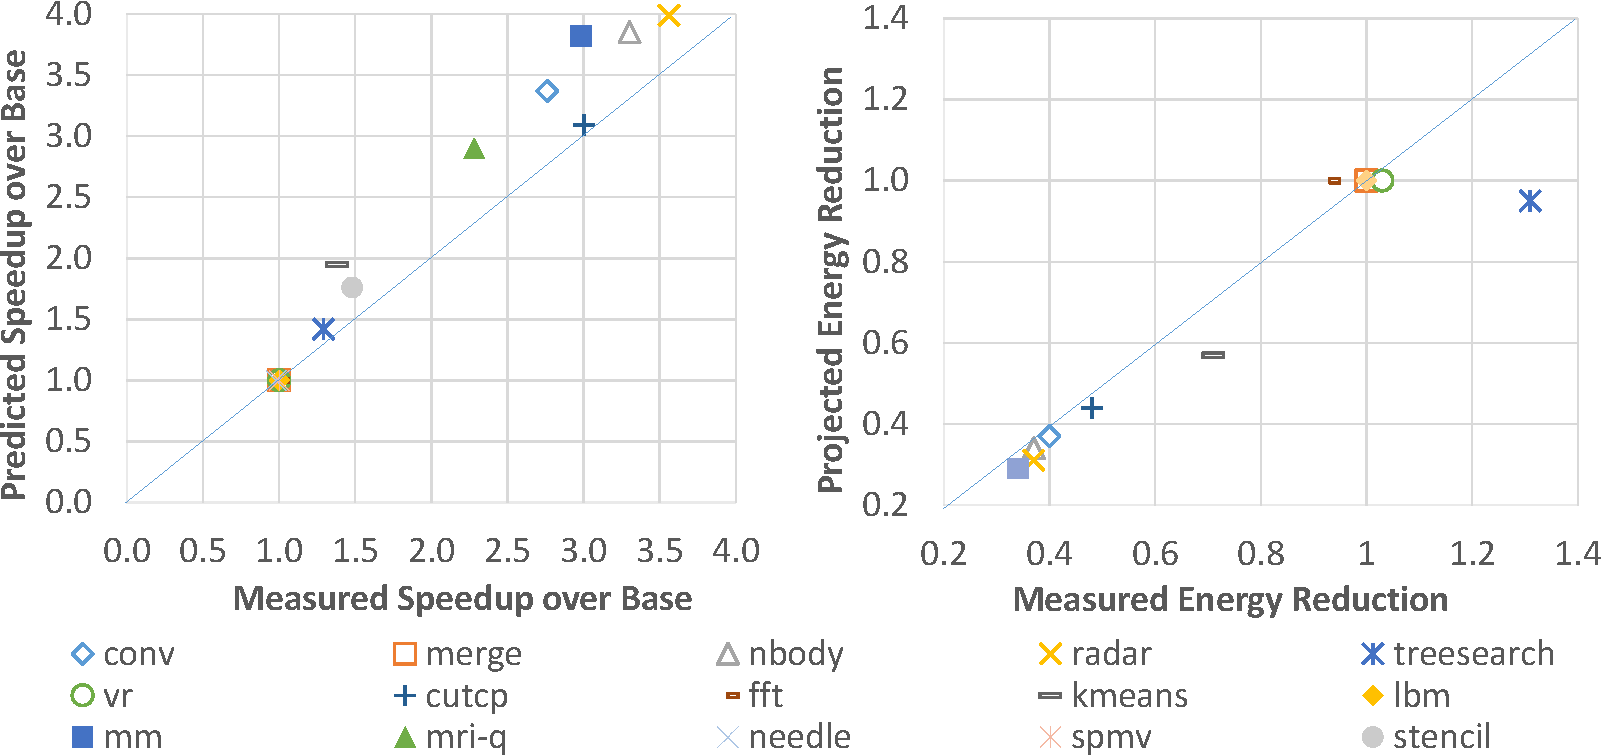
\includegraphics[width=0.44\linewidth]{figs/v_simd.pdf}} &
    \multicolumn{2}{ c }{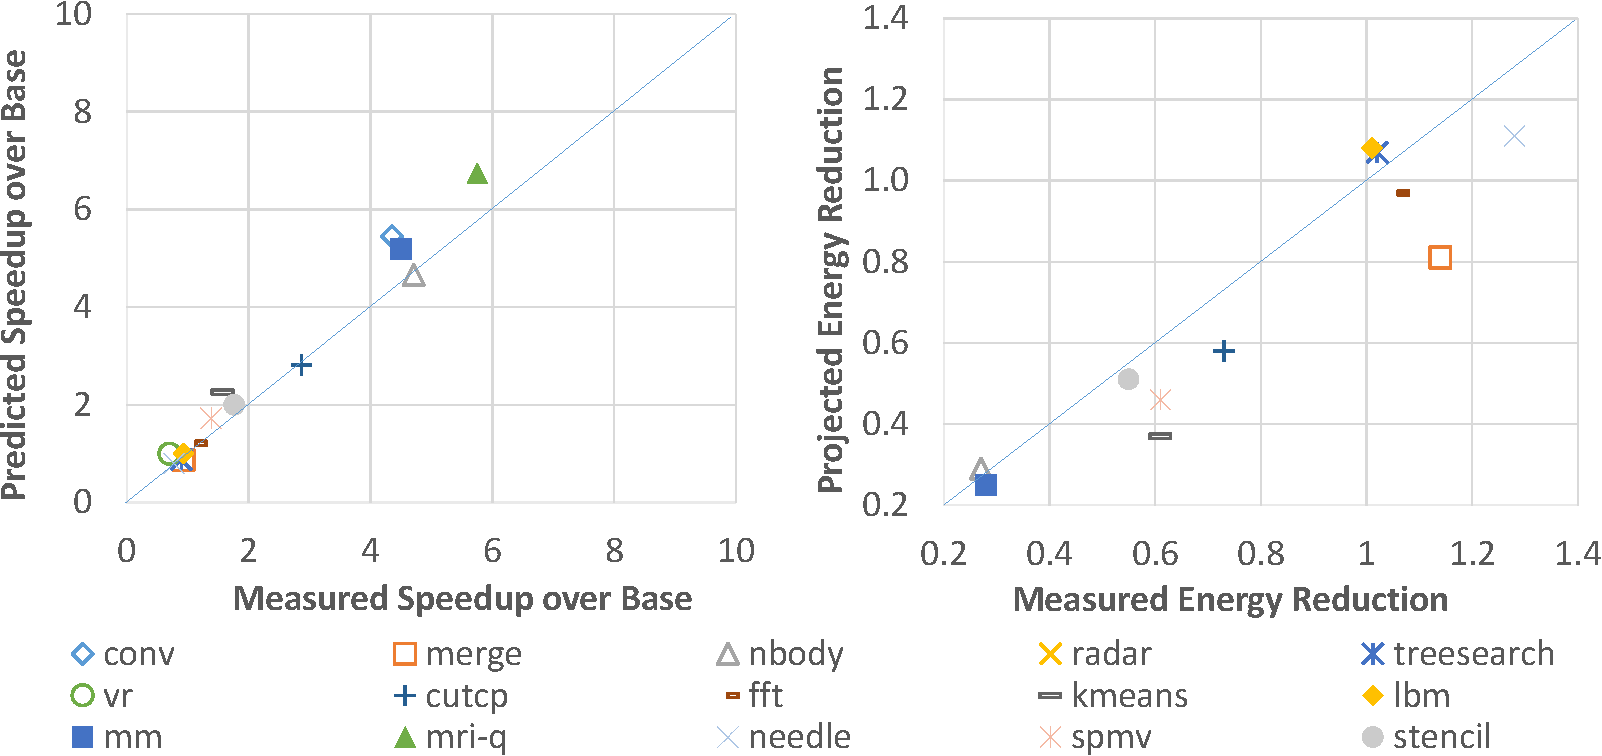
\includegraphics[width=0.44\linewidth]{figs/v_dyser.pdf}} \\
    \midrule

\end{tabular}
\end{center}
\vspace{-0.1in}
\caption{Prism Validation}
\label{fig:validation}
\end{adjustwidth}
\end{figure}



\subsection{Prism Validation}

\paragraph{Validation Methodology}  The benchmarks we use in this study come
from a combination of benchmarks used in the design evaluations from each
previous work.  They are listed in full in Table~\ref{tab:benchmarks}(on
page~\pageref{tab:benchmarks}).  For validating the accelerators, we chose
processor configurations which attempted to best match descriptions in
respective publications. BERET and C-Cores used a dual-issue, inorder CPU,
while the quad-issue DySER model used a quad-issue OOO 
CPU~\cite{ieeemicro12:dyser,Gupta:2011:BER:2155620.2155623,Venkatesh:2010:CCR:1736020.1736044}.  For validation with SIMD, we set the vector width at 4 words.  
Table~\ref{tab:omgvalidation} presents a summary of our validation benchmarks
and results.
%and Figure~\ref{fig:validation} shows the validation graphs
%for the OOO core and four accelerators. 

\paragraph{OOO-Core Validation Results}
To determine if we are over-fitting
the OOO core to our simulator, we perform a ``cross validation'' test: 
we generate a trace based on the 1-Wide OOO core, 
and use it to predict the performance/energy of an 8-Wide OOO core, and vice-versa.
Figures~\ref{fig:validation}(a) and ~\ref{fig:validation}(b) show the results respectively.
The benchmarks are an extension of those used to validate the Alpha 21264\cite{simalpha}.
%,summarized briefly in Table~\ref{tab:micro-benchmarks}.
The high accuracy here ($<4\%$ on average) demonstrates the flexibility of the model
in either speeding up or slowing down the execution. 

\paragraph{Accelerator Validation Results} 
Figures~\ref{fig:validation}(c-e) show the accelerator validation results.
Overall, for every accelerator, we
achieve an average absolute error of less than 15\%, both in terms of
performance and energy reduction, compared to simulator or published data.
Note that we do not have access to the NPU energy model, so no energy
validation is reported.

\begin{table}
\begin{center}
\footnotesize
\def\arraystretch{0.99}
\setlength{\tabcolsep}{.18em}

   \begin{tabular}{>{\RaggedRight}p{1.3in}>{\RaggedRight}p{1.4in}>{\RaggedRight}p{1.1in}rr}  \toprule

   \textbf{Accel.} & \textbf{Benchmarks} &  \textbf{Core Config} 
  & \textbf{P}  & \textbf{E}\\ \midrule

   8-Wide$\rightarrow$1-Wide
   & $\mu$bench\cite{simalpha}%, see Table~\ref{tab:micro-benchmarks}.
   & 1-Wide OOO
   & 3\%
   & 4\% 
   \\    

   1-Wide$\rightarrow$8-Wide
   & $\mu$bench\cite{simalpha}%, see Table~\ref{tab:micro-benchmarks}.
   & 8-Wide OOO
   & 2\% 
   & 3\%
   \\

   Conservation Cores   
   & Data/Bench from ~\cite{ccores}
   & 2-Wide Inorder 
   & 5\%
   & 10\%  
   \\

   BERET   
   & Data/Bench from~\cite{Gupta:2011:BER:2155620.2155623}
   & 2-Wide Inorder 
   & 8\%
   & 7\%
   \\

   SIMD
   & Data/Bench from~\cite{DBLP:conf/IEEEpact/GovindarajuNS13}
   & 4-Wide OOO
   &12\%
   & 7\%
   \\

   DySER
   & Data/Bench from~\cite{DBLP:conf/IEEEpact/GovindarajuNS13}
   & 4-Wide OOO 
   &15\%
   &15\%
   \\

   NPU
   & Data/Bench from~\cite{npu}
   & 4-Wide OOO 
   & 11\%
   &
   \\
    
\bottomrule
  \end{tabular}
\end{center}
\vspace{-0.22in}
  \caption{Validation Results, \textnormal{\footnotesize P: Avg Perf. Err, E: Avg En. Err}}
  \label{tab:omgvalidation}

\end{table}


\if 0
\paragraph{OOO Cross Validation}
We validate our out-of-order core model against the GEM5 simulator which we are basing
it off of.  To determine if we are over-fitting to the specific machine
parameters, we perform a ``cross validation'' test:  we generate a trace based on the
1-Wide OOO core, and use it to predict the performance and energy of an 8-Wide OOO 
core (and vice-verse).  The benchmarks we use are an extension of those which were
used to validate the Alpha 21264 for simple scalar\cite{simalpha}. Due to space 
constraints, we summarize these benchmarks briefly in Table~\ref{tab:micro-benchmarks}.
% Our basic strategy
%was to implement the micro-benchmarks from this paper, then add new micro-benchmarks
%to test incorrect modeling behavior observed in our applications.  
\fi

\if 0
\begin{table}
\begin{center}
\footnotesize
\def\arraystretch{0.9}
\setlength{\tabcolsep}{.21em}

    \begin{tabular}{l>{\RaggedRight}p{3.8in}}  \toprule
    \textbf{Prefix} & \textbf{What it Captures} \\ \midrule
    C & Control flow with varying predictability and squash penalties. \\
    D & Data parallel benchmarks with different operations.\\
    E & Execution latency\&b/w stressing benchmarks.\\
    M & Memory latency\&b/w stressing benchmarks.\\
    S & Benchmarks affecting store buffer effects.\\
    
\bottomrule
  \end{tabular}
\end{center}
\vspace{-0.22in}
  \caption{OOO Micro-Benchmarks}
  \label{tab:micro-benchmarks}
\vspace{-0.1in}
\end{table}
\fi

\if 0
The results of this experiment are shown in 
Figure~\ref{fig:validation} (a) and (b).  For performance, we show
the measured versus projected Instructions Per Cycle (IPC), and for energy,
we are showing the measured versus projected Instructions Per unit Energy (IPE).  For
these metrics, we have an average absolute error of 2\% and 3\% error respectively 
on the 1-Wide to 8-Wide test, and a 3\% and 4\% average absolute error for the 1-Wide to
8-Wide test.  Overall, our out-of-order core model is well within the noise 
margin for accuracy.

\paragraph{Conservation Cores Validation}
We validate our Conservation Cores model against the data from~\cite{ccores}, using
all five benchmarks shown in the paper, and show the results in
Figure~\ref{fig:validation}(c).  Here, the baseline core is a dual issue in-order core,
and we compare against our transformed graph for modeling inorder cores.
We achieve an average of 5\% and 10\% average absolute
error in terms of performance improvement and energy reduction.  The worst case is for
401.bzip2, where we under-predict performance by 15\%.  Even this may be within the
expected error range, considering that we do not have detailed access to the exact
baseline processor which was used in this study.

\paragraph{BERET Validation}
The BERET accelerator is validated against the data 
from~\cite{Gupta:2011:BER:2155620.2155623}, and the results are shown in 
Figure~\ref{fig:validation}(d).  Again, the baseline is a dual issue inorder core.
We achieve an average absolute error of 8\% and 7\% in terms of performance improvement
and energy reduction.  We over-predict performance slightly on cjpeg and gsmdecode,
likely because we do not constrain ourselves to fixed SEBs(compound functional units), 
and simply create subgraphs of size 5 (higher than the average of about 2.5 from the published data).

\paragraph{SIMD Validation}
For validation of the SIMD accelerator, we used the Gem5 Simulator's implementation,
configured as a 4-Wide OOO processor.
Figure~\ref{fig:validation}(e) shows how we attain an average absolute 
error of 12\% and 7\% in terms of performance improvement and energy reduction.
We remark that our predictions for SIMD are intentionally optimistic, as there
is evidence that compilers will continue to see improved SIMD performance as
their analysis gets more sophisticated~\cite{6113845}.  

\paragraph{DySER Validation}
For validation of the DySER accelerator, we used the used the Open Source
release of their tools. Figure~\ref{fig:validation}(e) shows how we attain 
an average absolute error of 15\% and 15\% in terms of performance improvement 
and energy reduction. Part of the reason we were able to match so well, at
least in terms of performance, was due to the insight gained through using
their toolchain.

\paragraph{NPU Validation}
We validate NPU model using the benchmarks, neural network topology
and results from Esmaeilzadeh et al.~\cite{npu}. We compute
the latency of a NPU computation using the neural network topology for
the corresponding benchmarks. We attain an average
absolute error of 11\% of performance improvement. (fft: 6\%,
inversek2j: 3\%, jmeint: 2%, jpeg: 10%, kmeans: 1% sobel: 53\%).
\fi


\subsection{Scope of the Transformable Dependence Graph} \label{sec:scope}
%Thus far, we have shown that the TDG works for a variety of different
%architectures, which each exploit different application properties, and
%have very different underlying micro-architectures.  That said, there
%are limitations to the TDG model with respect to the type of architecture
%it can model, and we attempt to elucidate these next.
Here we describe the limits of the TDG model in terms of coupling with the
general purpose core and algorithmic change.

\paragraph{Coupling}
The first dimension which we consider is the scope of is the coupling between
the accelerator and the general purpose processor.  Figure~\ref{fig:coupling}
outlines some examples, and four simple categories.  First are accelerators
like SIMD or DySER, which are tightly coupled to the GPP, which we call
``integrated''.  They do not have their own interface to the memory system, and
rely on the GPP.  In-core accelerators are those which completely eschew the
GPP, but still share the same memory port.  Off-core accelerators are those
which attach anywhere else inside the same memory system as the GPP, and
standalone accelerators don't require the GPP's memory system at all.

\begin{figure}[t]
\begin{center}
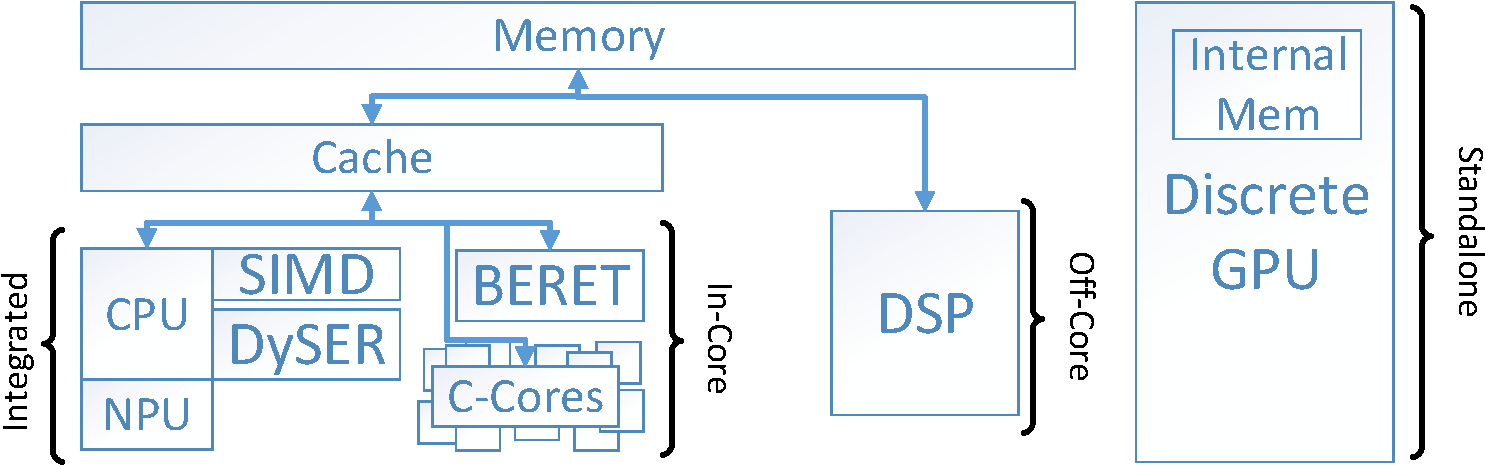
\includegraphics[width=0.7\linewidth]{figs/arch-scope.pdf}
\end{center}
\caption{Accelerator Coupling Classification}
\label{fig:coupling}
\end{figure}

In terms of coupling, we've already shown how in-core and integrated accelerators can
be modeled effectively.  Off-core and standalone accelerator's pose a
significant challenge, because it's difficult to determine how the change in
the interface to memory will affect the latency and bandwidth.  If the
interface to memory is simple, say that no caches are used, and the latency
is fixed, then modeling these types of architectures would be possible.
One second order error with this approach is that the offloading of certain computations
could affect what gets pulled into cache, and therefore the modeling of the GPP's
memory accesses would be somewhat inaccurate if the accelerator and GPP share
memory at a fine granularity. 

A tractable solution to the problem would be to attach a memory
system simulator to the TDG model.  This is largely unsatisfying, though, as it
would lessen the degree of ``purity'' of the TDG's graph based model, which is
arguably it's foremost strength.  Another potential direction is to use
statistical techniques to stochastically model the memory system interaction,
but this would likely introduce a significant source of error.  Overall, it's
an open question how effective the TDG could be for modeling off-core and standalone
accelerators.

\paragraph{Algorithm}
Certain accelerators, like GPGPU's, require fundamental changes to the
algorithm of the program to be effectively employed.  For example, an effective
GPU histogram bears very little resemblance to its simplistic CPU counterpart.
Unless this algorithmic change can be modeled as a graph transformation, then
the TDG cannot model this architecture.  One example of program modifications
that can be modeled is that of loop vectorization, which can be done because
it's straightforward to coalesce loop iterations in the TDG.  However, the
broader class of algorithmically different accelerators is challenging, and
this is why we posit that accurate TDG models for their architectures,
including GPUs, will remain elusive.

Interestingly, for certain classes of accelerators, like the NPU, some degree of
modeling is possible.  This is because we can determine through external methods
what the accelerator's internal behavior is.

\paragraph{Computation/Data Specific Optimizations}  
Finally, certain classes of accelerators take advantage of the specific
computations and data in order to simplify the hardware.  One prominent example
of this is to reduce the data-width (or bit-width) to be a size just large
enough to fit the data.  This could potentially result in significant energy
savings.  This type of optimization could be capture by the TDG if we added
value tracking, and developed an energy model for specialized operations.  
Though modeling computation/data specific optimizations could be
useful, we have not pursed them further as no accelerator's we've evaluated so
far has required them.

